\chapter{2020-06-16}
\textbf{Checklist}
\begin{enumerate}
    \item \faCheckSquareO Performance gap between valid and test. \\ 
    Give a better explanation about why alignment results on test is still better than valid. (The candidates for valid is half less than the test, but the valid mrr is still lower than the test.)

    \item \faTimesCircleO Relation classification is still overfitting.
    %\begin{enumerate}[label*=\arabic*.]
    \begin{enumerate}
        \item \faCheckSquareO Try applying a dropout to the output of hidden layer, not only just the input of hidden layer.
        \item \faCheckSquareO Try adding more hidden layers.
        \item \faCheckSquareO Try lowering the ratio and scale of $\beta_1$ for relation cross entropy loss.  
    \end{enumerate}

    \item KG completion evaluation 
     \begin{enumerate}
        \item \faCheckSquareO Check the code for evaluating on KG completion
        \item \faCheckSquareO Use the overall loss for early stopping instead of only the hits1 on alignment
        \item \faCheckSquareO Figure out why completion results (hits@N, mrr, mr) are pretty bad, why it's much worse than alignment (why completion task is harder than alignemnt task).
    \end{enumerate}

    \item \faCheckSquareO Make sure the baseline is all good. Compare the model with or without relation calssifier.
    \item Draw the heatmap for $\beta_1$ and $\beta_2$ with rel\_acc and mrr.
    \item \faCheckSquareO Make sure the test data is not used for training.
    \item Pre-train the relation-classifier and then freeze it to train other parts of models. 
    \item Design better negative sampling strategies. 
\end{enumerate}

\section{Overfitting on relation classification}
Now the relation classifier is a three layers of FNN. 
When I tried to dropout the inputs of the first and second layer, it indeed can prevent the overfitting when the dropout rate is set to 0.8 or 0.9. But too much dropout caused the the 'NAN' incidently and interrupt the training. This is because the relation types are accidently all set to zero.
So I have to reduce the dropout rate, and then the overfitting on appeared again. (Still need to try some other ways.)

\section{Performance Gap between Valid and Test}
The performance (mrr and hits) gap on alignment task between the valid set and test set is caused by the sampling order. \textbf{When first created them, I sampled the test set first, and then sampled the valid set.} The sampling process tends to sample the entities with higher frequency, which caused the frequencies in valid set is much higher than test set. Entities with higher frequency are easier for model to learn a better embedding, and thus leads to higher alignemnt performance. 
For entities on valid and test, I visualized them frequency distribution in both the overlap\_subset, ConceptNet and SWOW. 


\begin{figure}[!ht]
    \centering
    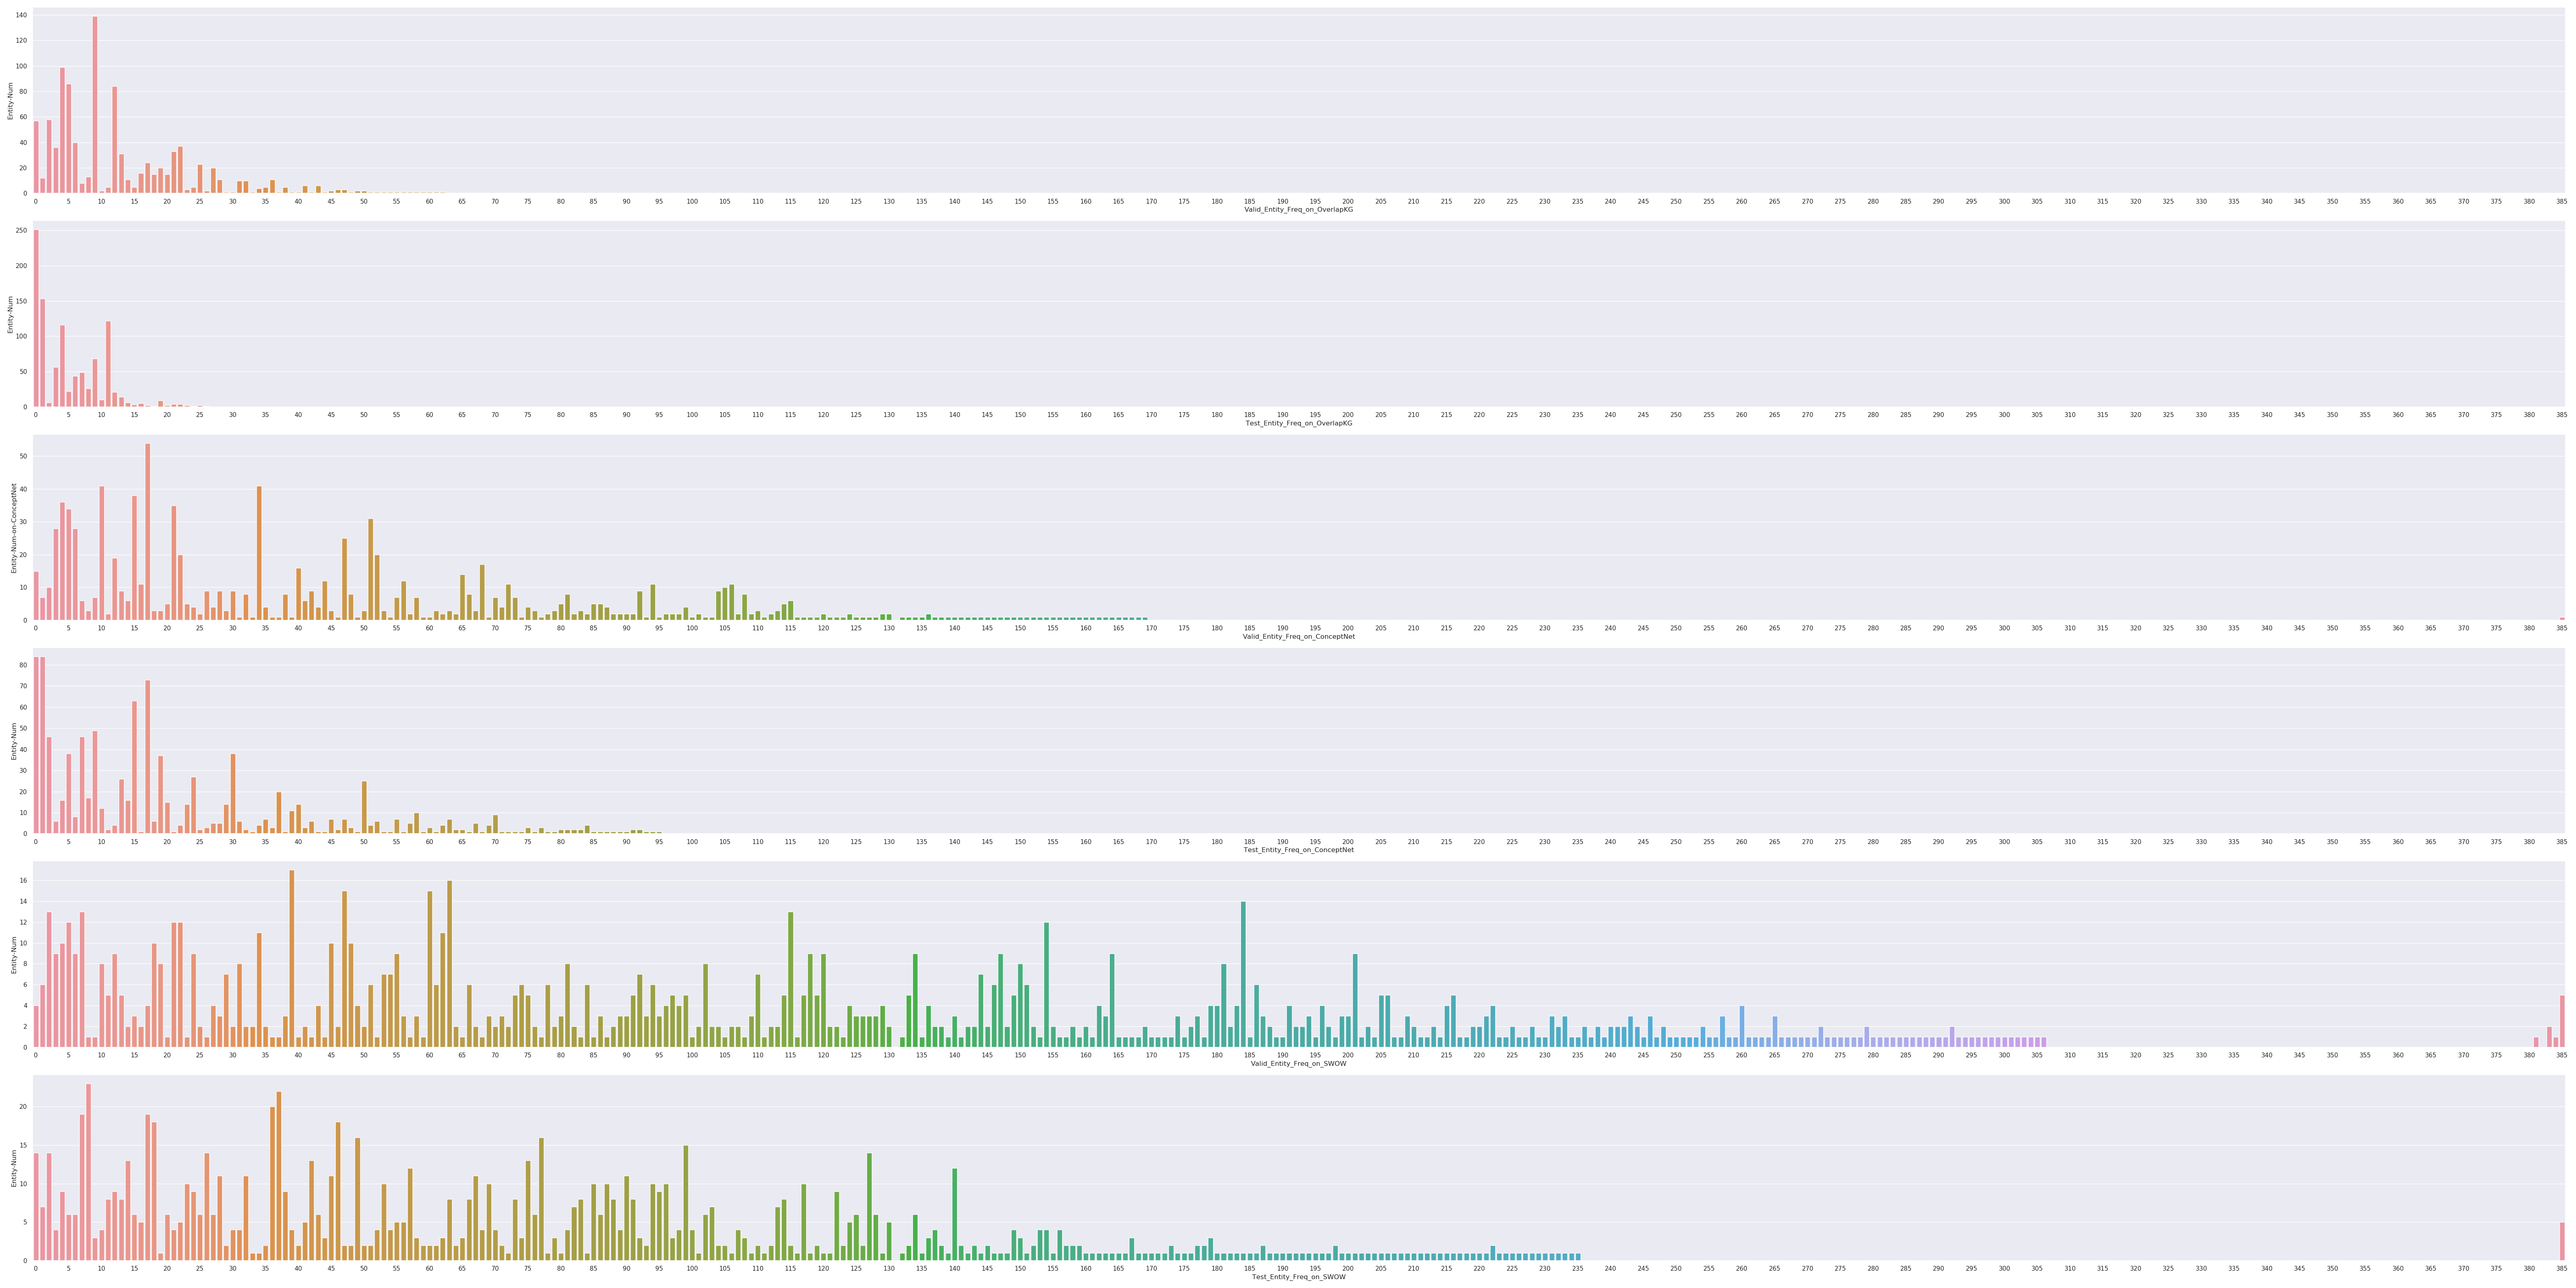
\includegraphics[width=\textwidth]{images/0616/C_S_V4_valid_test_ent_freq_distributions.png}
    \caption{\label{fig:biased_valid} Biased to valid: sample valid first. The odd row for valid and the even row is for test.}
\end{figure}
\begin{figure}[!ht]
    \centering
    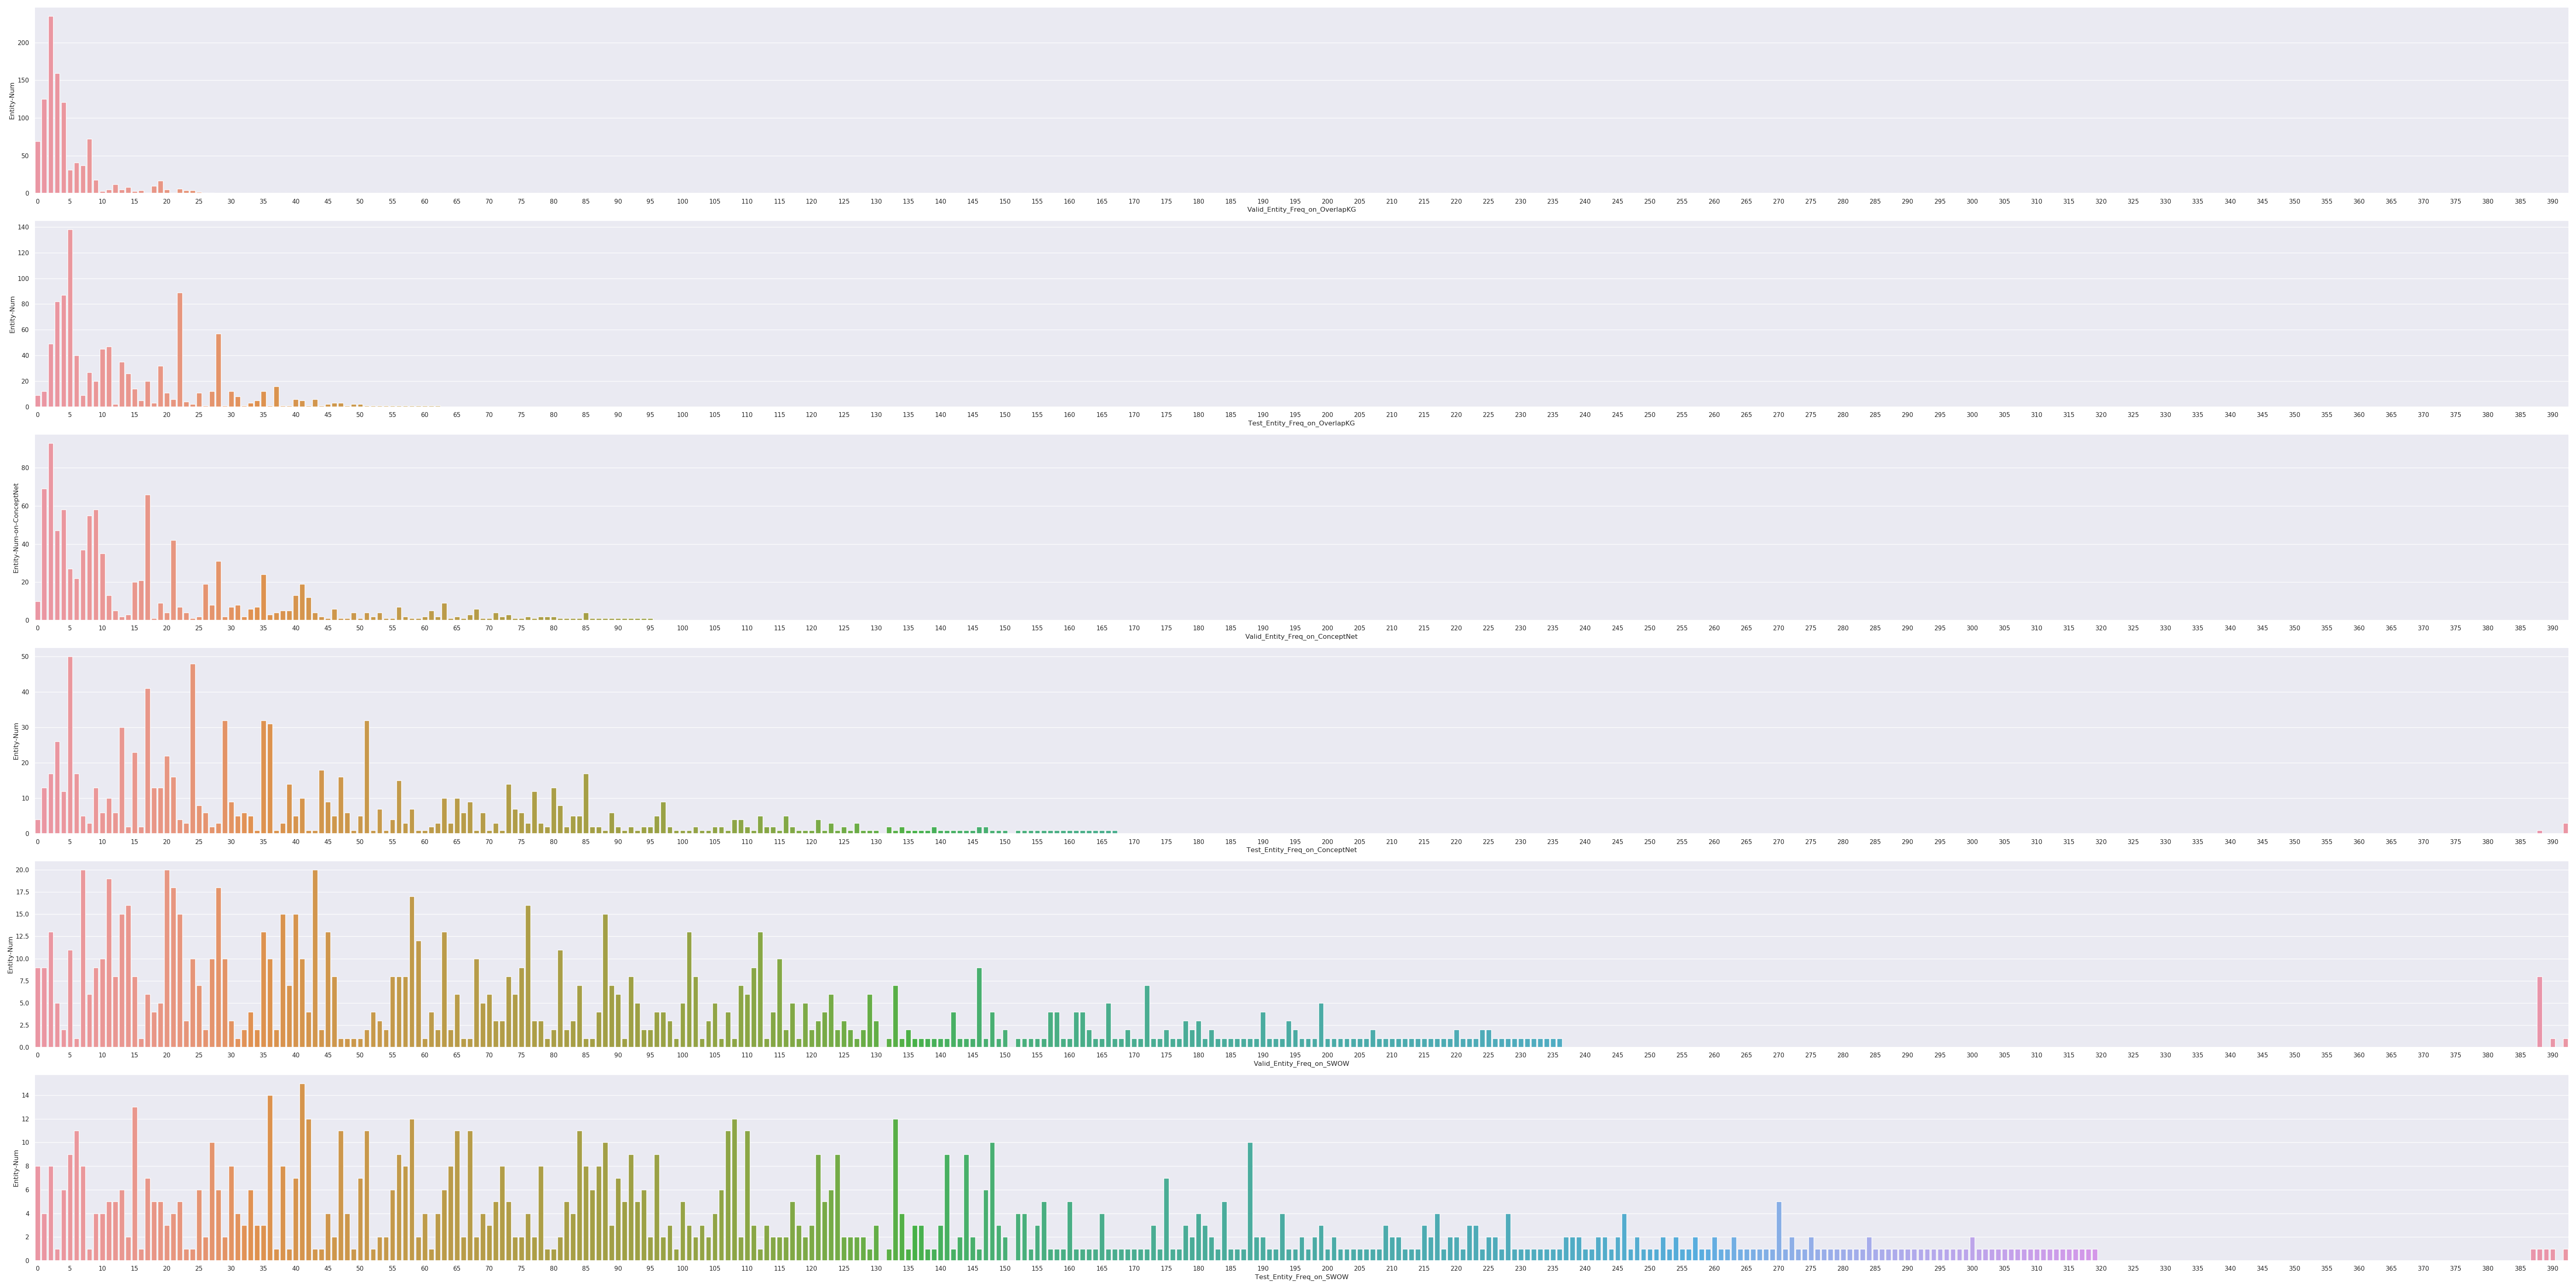
\includegraphics[width=\textwidth]{images/0616/C_S_V5_valid_test_ent_freq_distributions.png}
    \caption{\label{fig:biased_test} Biased to test: sample test first. The odd row for valid and the even row is for test.}
\end{figure}
\begin{figure}[!ht]
    \centering
    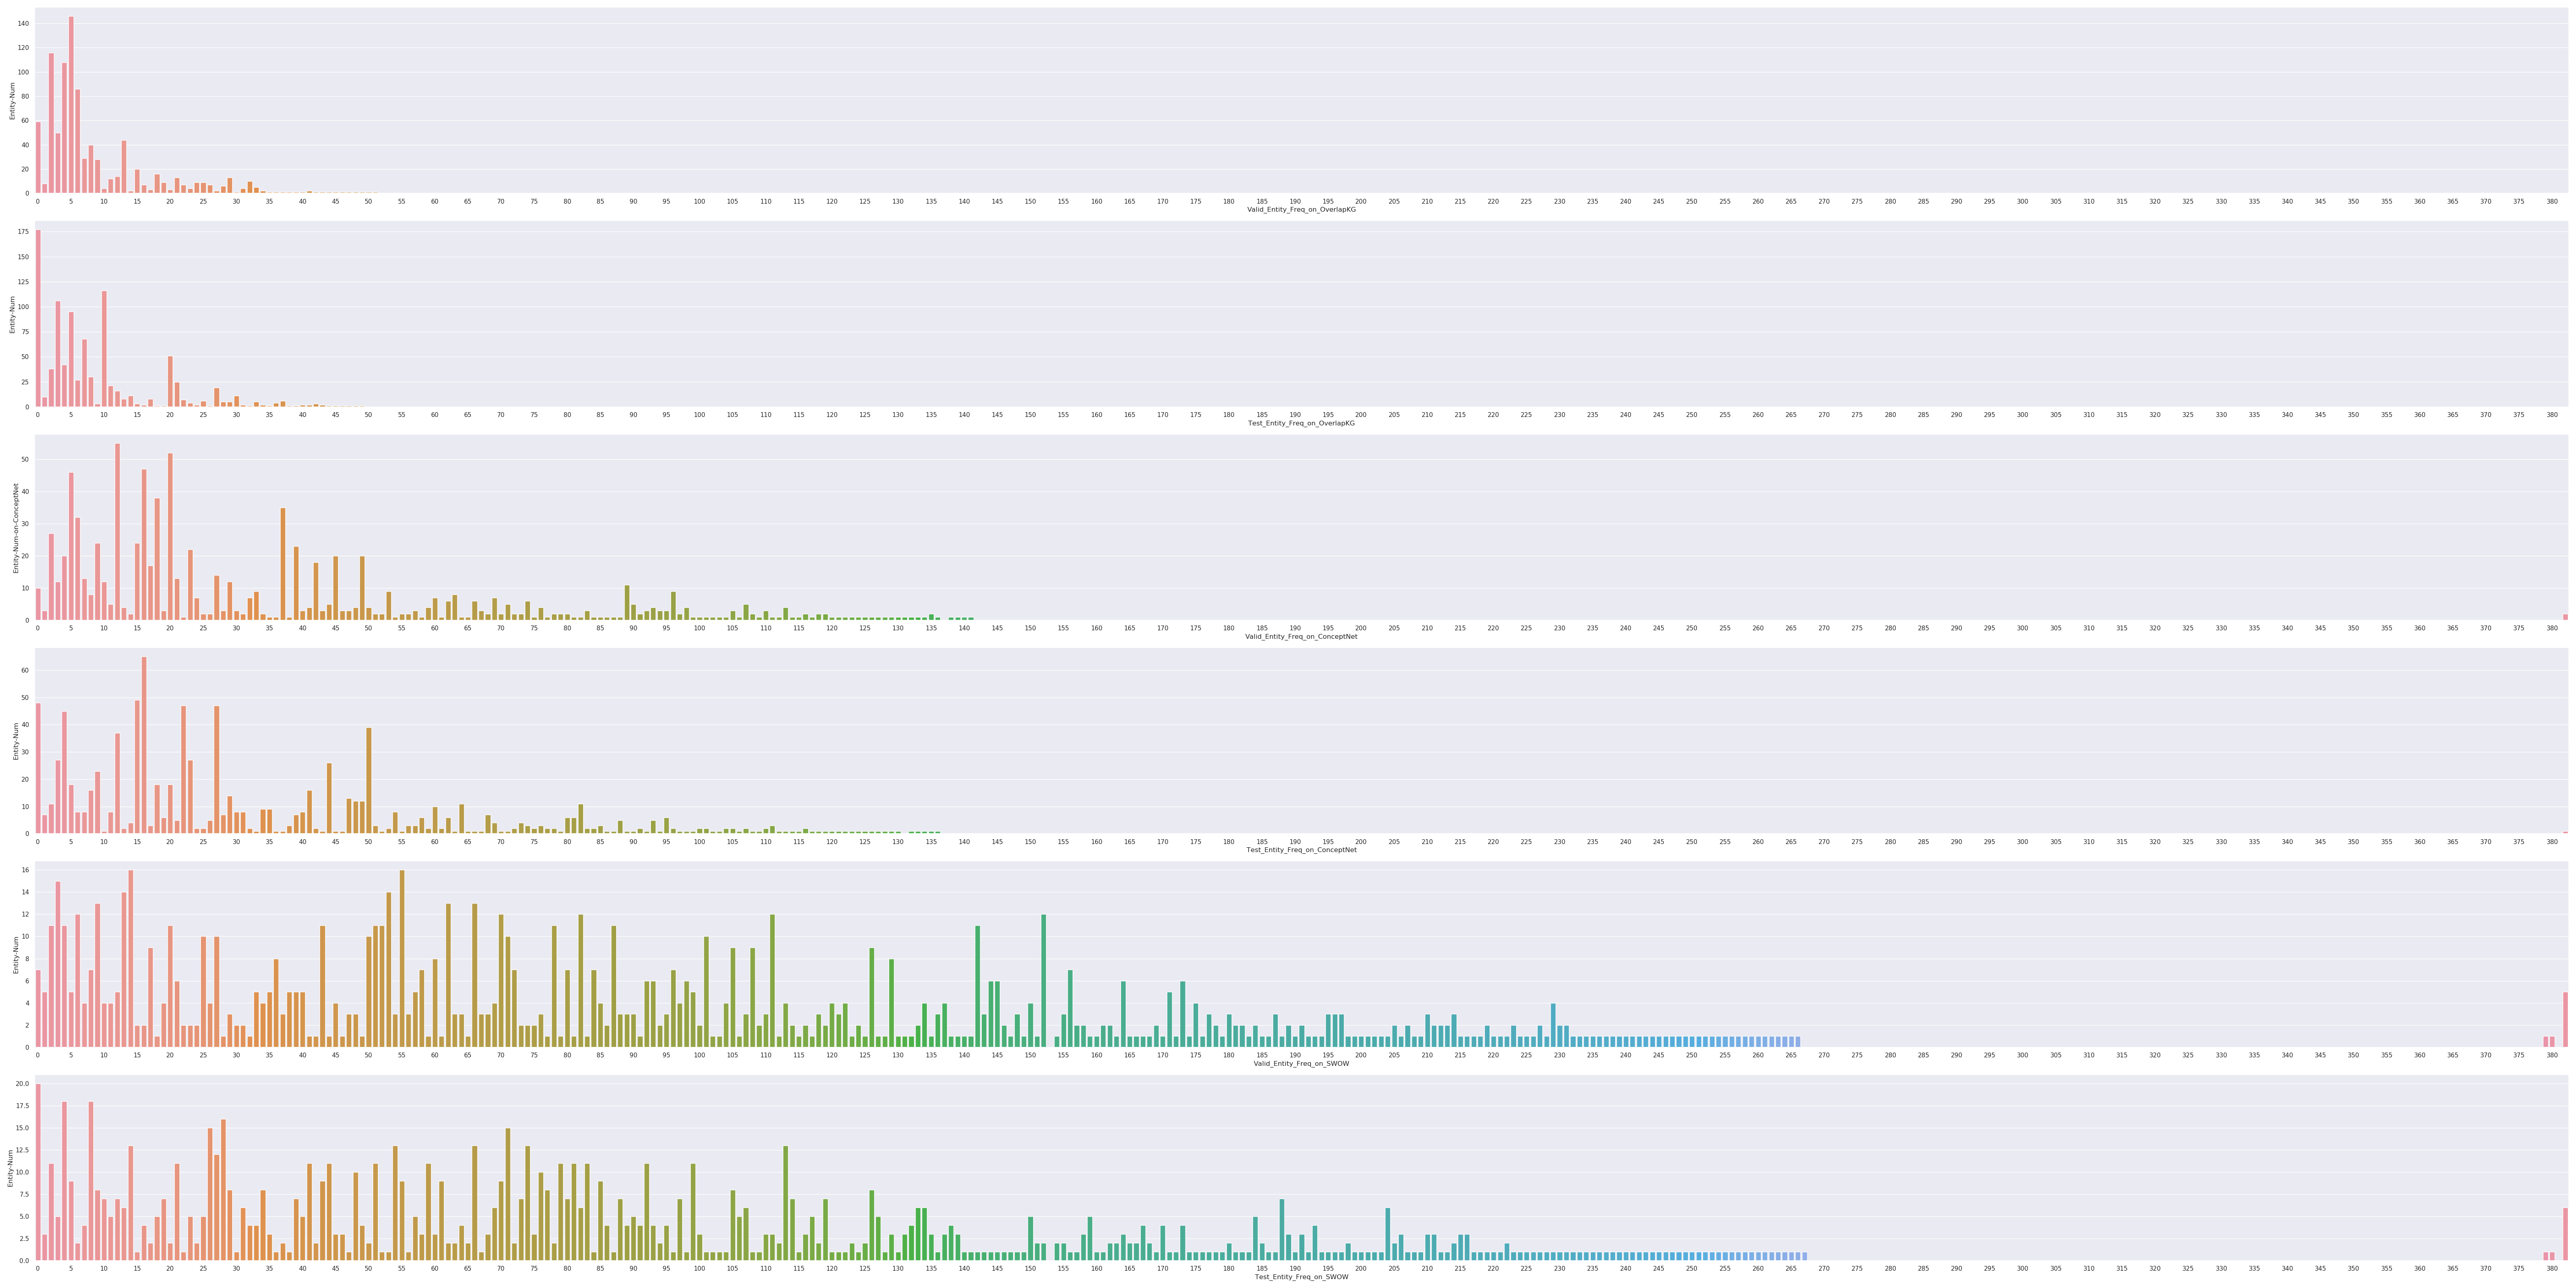
\includegraphics[width=\textwidth]{images/0616/C_S_V6_valid_test_ent_freq_distributions.png}
    \label{fig:unbiased_valid_test_ent_freq_distributions}
    \caption{Bias reduced sample: sample valid and test iteratively with a number of min-batch. The odd row for valid and the even row is for test.}
\end{figure}
By comparing the three frequency distributions, we can see that entities sampled first have higher frequency and infer higher frequency entities leads to better evaluation performance.  
I also compared the alignemnt-mrr curves for valid and test during trining process and testified this hypothesis (see figure ~\ref{fig:comparision_of_different_sample_valid_test_order}).

%The Figure~\ref{fig:biased_valid}, 
Figure~\ref{fig:biased_test}, and Figure~\ref{fig:unbiased_valid_test_ent_freq_distributions} show the frequency distribution for entities in the valid and test. 
The x-axis is the frequency of a entity, the y-axis is the entity num with correspoing frequency in the test/valid set. Figure~\ref{fig:biased_valid} is the frequency distributions of sampling valid first and Figure~\ref{fig:unbiased_valid_test_ent_freq_distributions} is the frequency distributions by sampling valid and test iteratively with a min-batch sample size to minimize the gap between them. Also, to control the influence of total rank candidates number, I tried to keep the overall entity number in the valid and test to be close (see Table~\ref{tab:statistics_two_versions_valid_test}).

\begin{figure}[!ht]
    \centering
    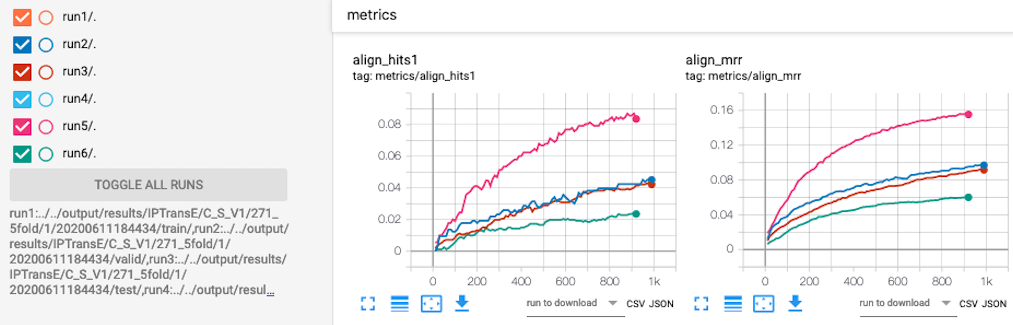
\includegraphics[width=\textwidth]{images/0616/comparision_of_different_sample_valid_test_order.png}
    \caption{\label{fig:comparision_of_different_sample_valid_test_order} Comparsion of biased and unbiased sample. The pink and green curves are the biased valid and test (sample valid first). The blue and orange curves are the unbiased valid and test. The gap between the unbiased are much smaller. }
\end{figure}

\begin{table}[H]
    \centering
    \begin{tabular}{cccc}
        \hline
        Version &Dataset & \#Triples &\#Entities \\
        \hline
        previous & valid & 565	&742\\
        previous & test & 1,236	&1,521\\
        \hline
        current & valid & 778	& 914\\
        current & test & 769	& 957\\
        \hline
    \end{tabular}
    \caption{\label{tab:statistics_two_versions_valid_test} Statistics for two different versions of valid and test.}
    
\end{table}

\clearpage
\section{Experimental Results}
Our hypothesis is joinly train ConceptNet and SWOW could possibly learn a knowledge shared embedding matrix for them. 

\subsection{Baselines}

\begin{figure}[!ht]
    \centering
    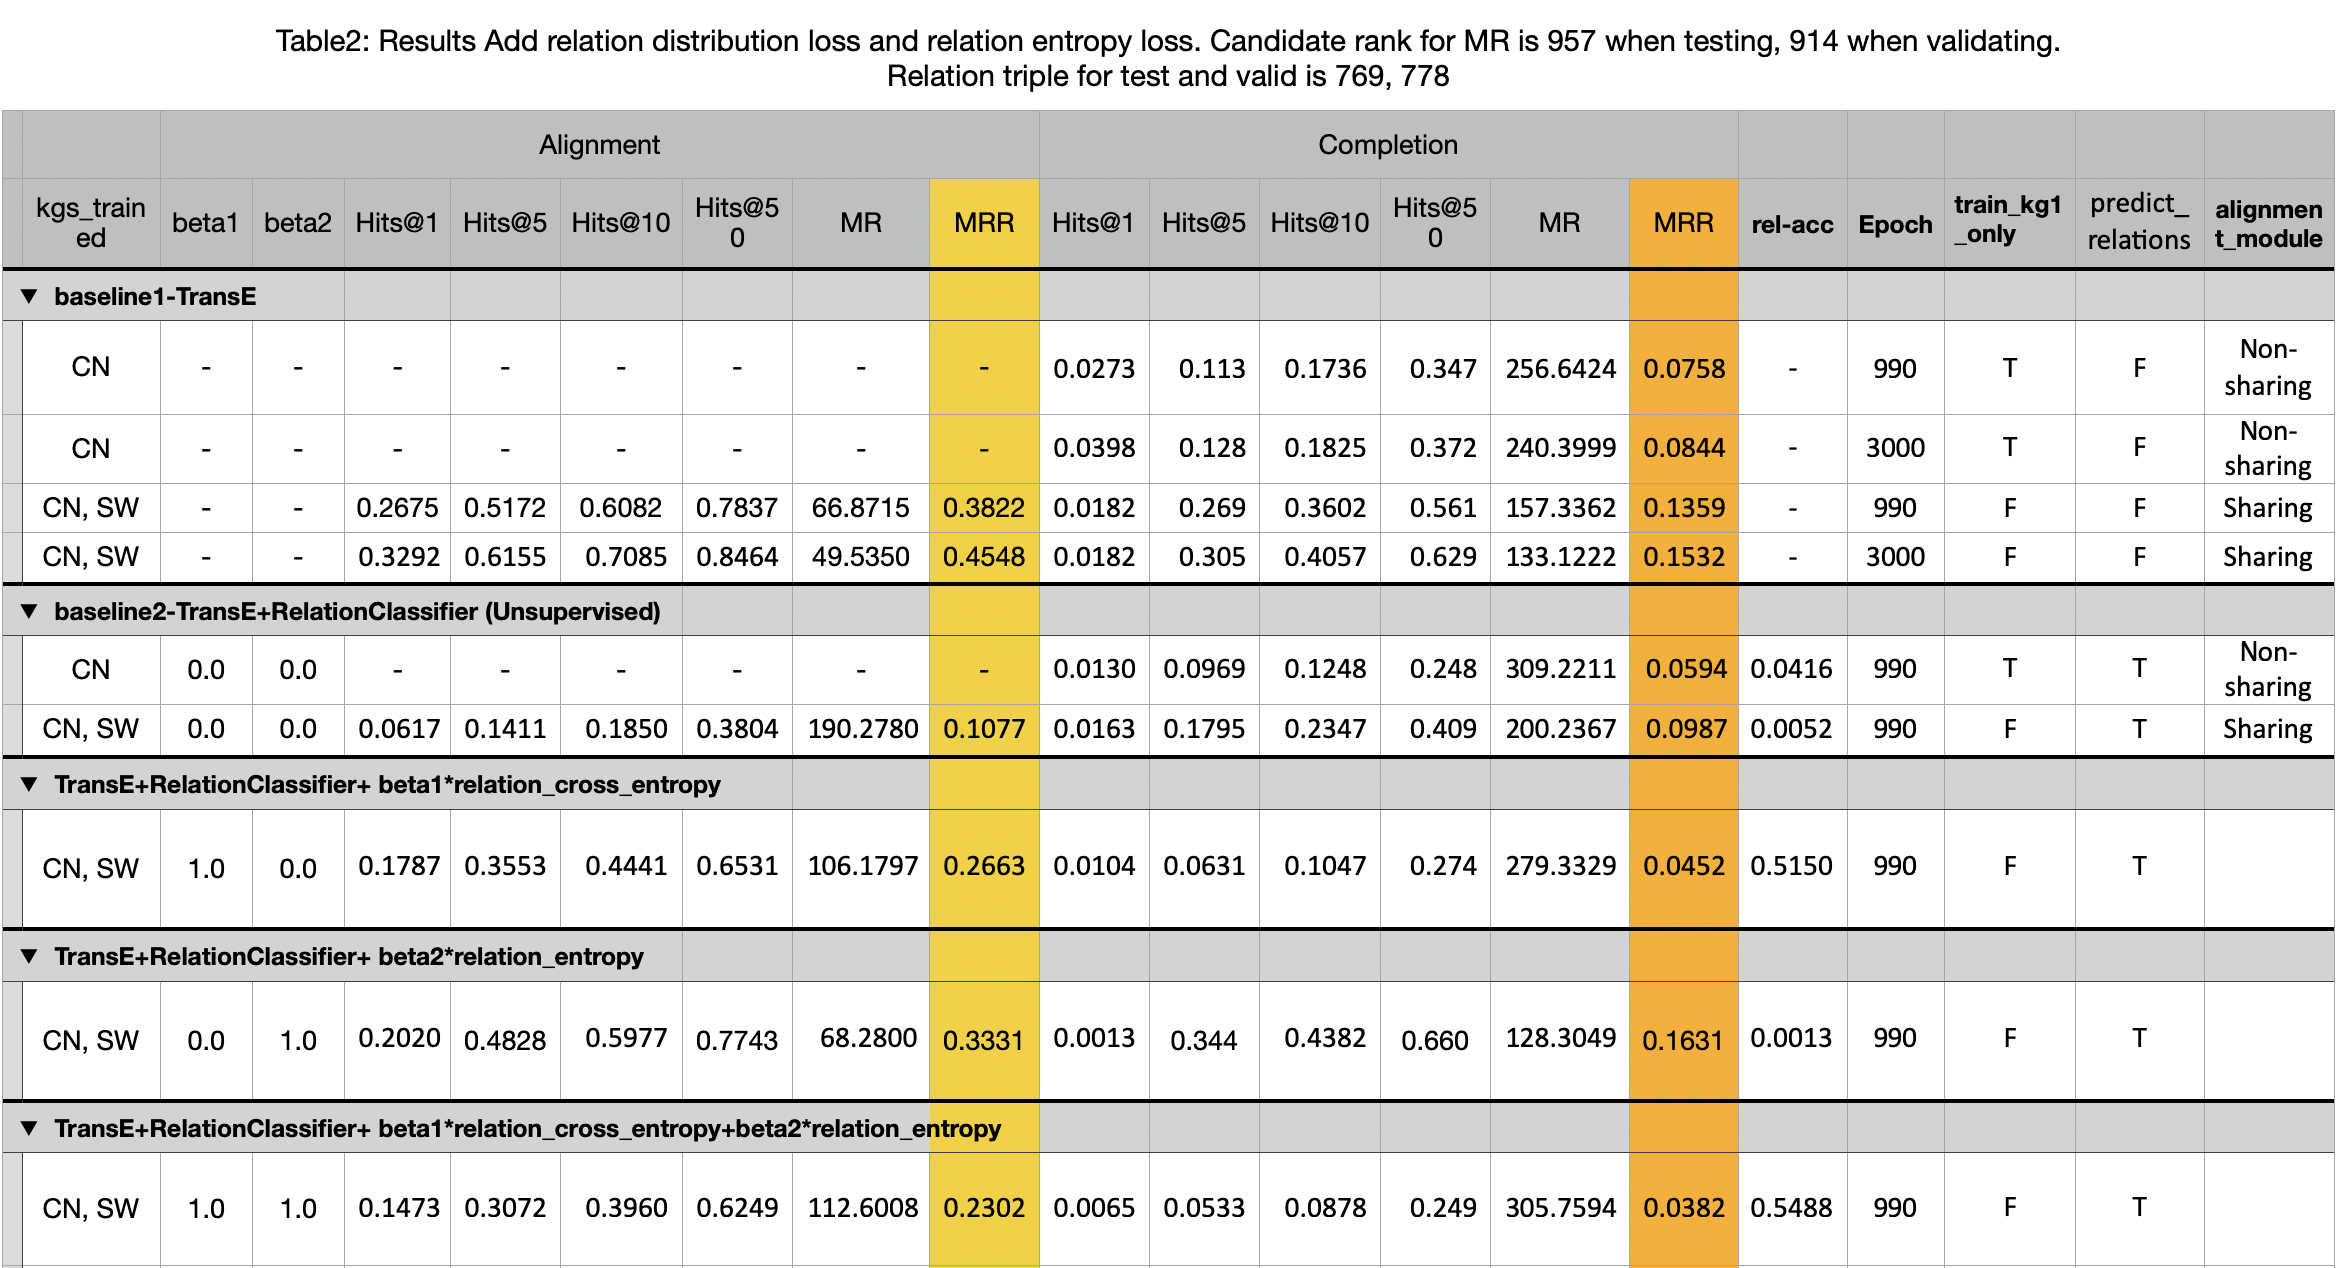
\includegraphics[width=\textwidth]{0616/baseline_results.png}
    \caption{Baseline Results}
    \label{tab:baseline_results}
\end{figure}
Observations from Figrue~\ref{tab:baseline_results}:
\begin{enumerate}
    \item Compare the results of baseline1-TransE, we can see the joinly training of ConceptNet and SWOW indeed help the completion on their overlap triples. Also, the MRR is increasing with the increase of trainig time when jointly train them. 
    \item When adding the relation calssifier into the model without relation type supervision, the performances dropped a lot, especially on the alignemnt task. This may suggest that the relation type is important for the learning of entity embeddings. 
    \item When the cross entropy loss is added on TransE loss, the accuracy of relation classification raises to 0.5150. The alignemnt MRR goes up but the completion MRR keeps going down.  
    \item When the entropy loss is added to constrain the relation distributions, the alignemnt MRR go back to the same level as the baseline1-TransE, and the completion MRR achieves even higher score than baseline1-TransE. Also, with supervison, the relation classification accuracy declined. This result is very interesting. It shows the model can learn good entity embeddings even when the relation types are not correctly predicted. This is contrary to our intuitive. Our intuition is when model gives better relation predictions, it'll give better results on alignment and completion tasks.
\end{enumerate}

\clearpage
\subsection{Correlations between beta1,beta2 and metrics}
%\textbf{Correlations between $\beta_1$, $\beta_2$ and metrics}

\begin{figure}[!ht]
    \centering
    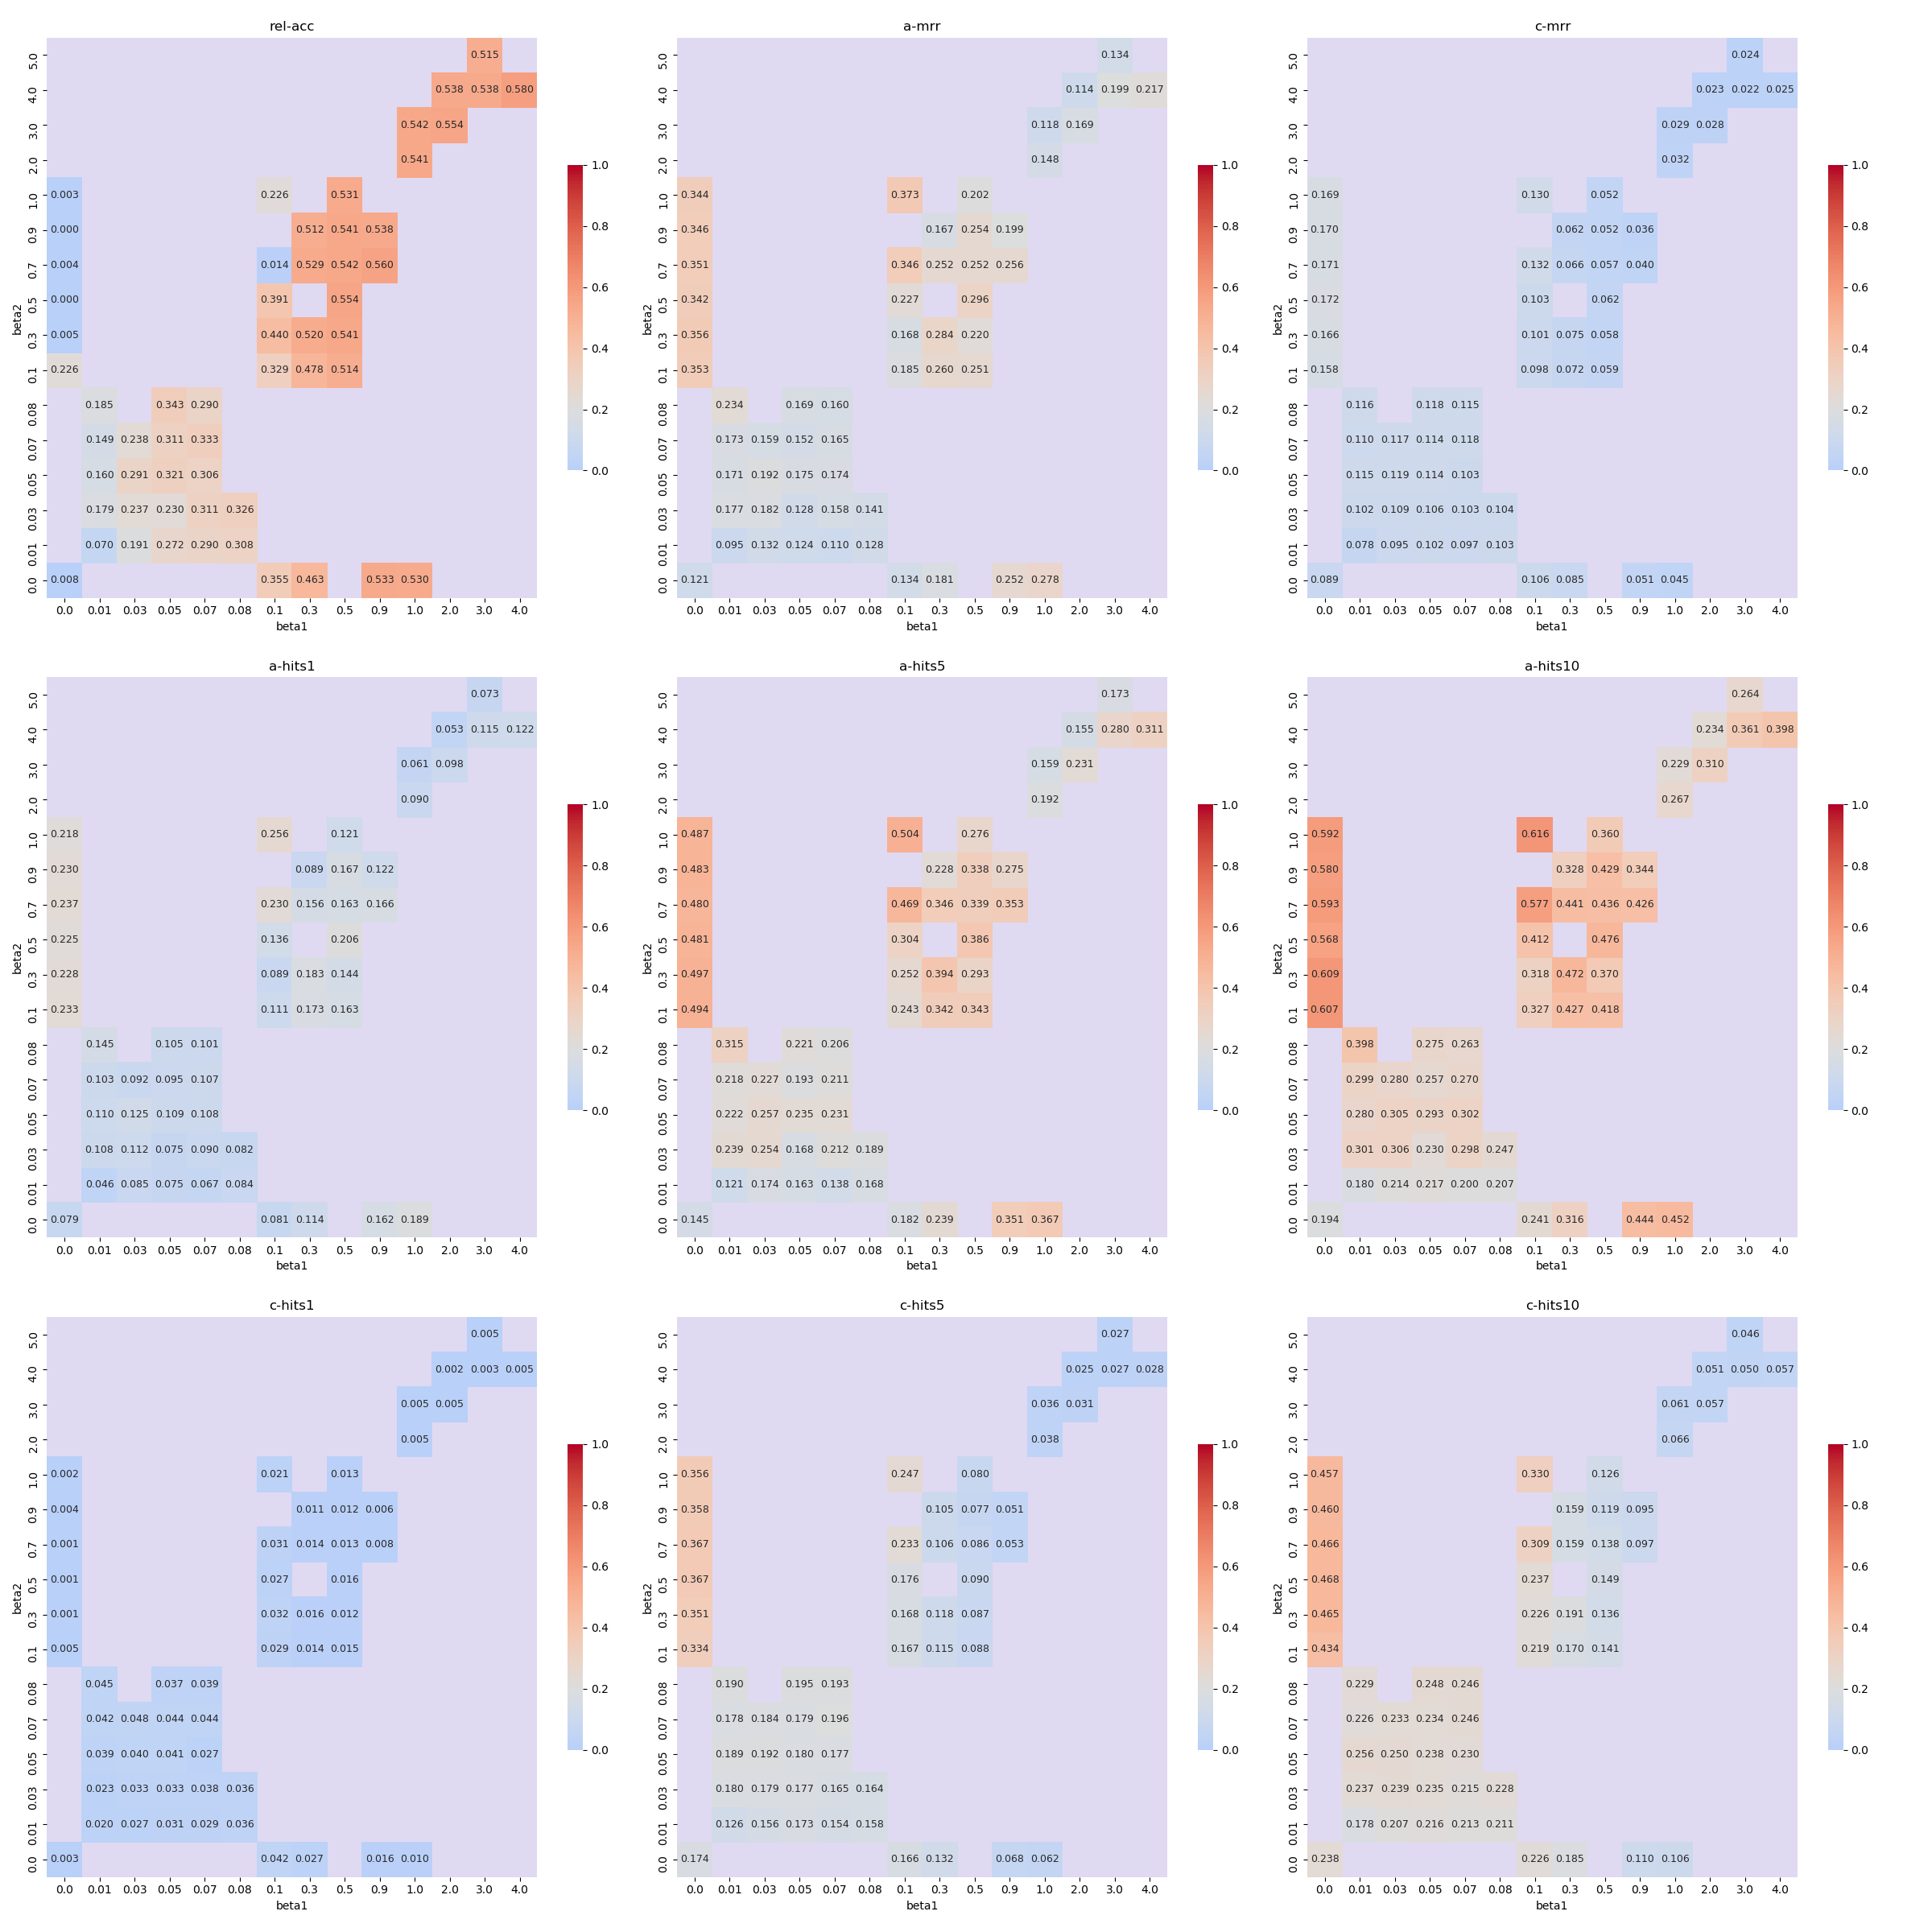
\includegraphics[width=\textwidth]{0616/heatmap_metrics.png}
    \caption{Relations between $\beta_1$, $\beta_2$ and various evaluation metrics.}
    \label{fig:heatmap_metrics}
\end{figure}
From Figure~\ref{fig:heatmap_metrics} can be seen that when $\beta_1$ is around 0.1, all the metrics look normal. But when increasing the $\beta_1$, e.g., $\beta_1 = 0.3$, the c-mrr would fall into very small value. However, the rel-acc is better when the $\beta_1$ is larger. The balance between them still needs to explore.

\clearpage
\section{Meeting Notes}
\textbf{Long term to do list}
\begin{enumerate}
    \item Find smarter negative sampling strategies.
\end{enumerate}

\noindent\textbf{Next week to do list}
\begin{enumerate}
    \item \faCheckSquareO Figure out why `NAN' appears during training. \\
        A: the scores for some relation types are too small and caused the underflow when apply log function to them. A small number 1e-9 is added to the scores for numerical stable.
    \item Debug the relation classifier \\
    For now, when $\beta_1$ is increased, the relation prediction accuracy become higher, but the alignment and completion performances dropped.  Try to figure out why, the code problem or the idea problem?
    Try to make the model and task to be simple to debug the relation classifier. 
    \begin{enumerate}
        \item \faCheckSquareO Lea: ``I was suggesting to come up with simpler variants (a toy data set, or limiting labels to only 2 classes) and see if your model behaves more meaningfully in these simplified scenarios... It may point you to issues with the implementation, or data set."
        \item Observe some prediction outputs for alignment rank, completion rank, and relation prediction (both training and valid). 
    \end{enumerate}
    
    \item Relation classification overfitting: try different training strategy to alleviate the problem. 
    \begin{enumerate}
        \item \faCheckSquareO Play with hyperparameters: lr, batch\_size, and training\_epoch. 
        \item \faCheckSquareO Pretrain the relation classifier.
        \item \faCheckSquareO Train the relation classifier every K ($K$ \textgreater $1$) iterations instead of every iteration. 
    \end{enumerate}

\end{enumerate}
papers lea has sent to me:
https://www.ijcai.org/Proceedings/2018/0581.pdf
https://www.ijcai.org/Proceedings/2019/0733.pdf

